% tlmgr install ...
\documentclass{article}
\usepackage{graphicx} % Required for inserting images
\usepackage{wrapfig}
\usepackage{amsmath} % Required for some math elements
\usepackage{mathtools} % Required for \coloneqq command
\usepackage[margin=2cm]{geometry} % Set margins to 2cm
\usepackage[danish]{babel} % Set language to Danish
\usepackage{tocloft}
\usepackage{cancel}
\usepackage{csquotes}
\usepackage{xcolor}
\usepackage{nicematrix}
\usepackage{caption}
% Required package
\usepackage{tikz}
\usetikzlibrary{positioning}

% Input layer neurons' number
\newcommand{\inputnum}{3} 

% Hidden layer neurons' number
\newcommand{\hiddennum}{5}  

% Output layer neurons' number
\newcommand{\outputnum}{2} 

\usepackage[
  style=apa,
  sortcites=true,
  sorting=nyt,
  backend=biber,
  autocite=inline
]{biblatex}
\addbibresource{paper.bib}

\renewcommand\cftsecfont{\normalfont}
\renewcommand{\cftsecleader}{\cftdotfill{\cftsecdotsep}}
\renewcommand\cftsecdotsep{\cftdot}
\renewcommand\cftsubsecdotsep{\cftdot}
\renewcommand\cftsubsubsecdotsep{\cftdot}

\newcommand{\figureref}[1]{Figur \ref{#1}}


\newcommand\Ccancel[2][black]{
    \let\OldcancelColor\CancelColor
    \renewcommand\CancelColor{\color{#1}}
    \cancel{#2}
    \renewcommand\CancelColor{\OldcancelColor}
}


\makeatletter
\newcommand{\subject}[1]{\gdef\@subject{#1}}
\newcommand{\class}[1]{\gdef\@class{#1}}
\newcommand{\mentor}[1]{\gdef\@mentor{#1}}
\renewcommand{\maketitle}{\bgroup\setlength{\parindent}{0pt}
\begin{flushleft}
  \textbf{\@title}

  \@subject\\\vspace{1em}
  \@author\\
  \@class\\
  \@date\\\vspace{1em}
  Vejledere:\\\@mentor
\end{flushleft}\egroup
}
\makeatother

\title{\Huge{Studie Område Projekt}}
\subject{Matematik A / Programmering B}
\author{Victor Østergaard Nielsen}
\class{3di - H. C. Ørsted Gymnasiet Lyngby}
\date{15/12/2024}
\mentor{Jan Strauss Hansen (Matematik A) \\ Kristian Krabbe Møller (Programmering B)}

\begin{document}

\maketitle
\newpage

\tableofcontents
\newpage

\section{Opgaveformulering}
\textbf{Machine-learning}\\\\
\textbf{Hovedspørgsmål}: Hvordan kan et simpelt neuralt netværk, uden unødige abstraktioner eller biblioteker, anvendes tilgenkendelse af håndskrevne tal i realtid i et tegneprogram på computeren, og hvad er matematikken bag?\\\\
\textbf{Opgaveformulering}:\\
\begin{itemize}
  \item Redegør overordnet for begrebet neuralt netværk.
  \item Redegør for de grundlæggende matematiske principper bag neurale netværk herunder matriceregning.
  \item Redegør for valg af programmeringssprog ift. udvikling af programmer med neuralt netværk.
  \item Analysér hvordan et neutralt netværk kan programmeres, gerne uden unødvendige abstraktioner eller biblioteker, så det kan genkende håndskrevne tal i realtid i/fra et tegneprogram på computeren.
  \item Undersøg hvorledes programmet kan optimeres for at opnå lavest mulig fejlrate og evt. hvorledes støj i den analyserede data kan påvirke fejlraten.
  \item Diskuter og vurder hvorvidt neutrale netværk er den mest effektive tilgang til at genkende håndskrevne tal på en adaptiv og robust måde.
\end{itemize}

\newpage
\section{Indledning}


\newpage
\section{Matricer og matrixregning}
\subsection{Matricer}
En matrice er en tabel af tal, der er arrangeret i rækker og kolonner. En matrice kan repræsenteres med et stort bogstav, f.eks. $A$, og elementerne i matricen kan repræsenteres som $a_{ij}$, hvor $i$ er rækken og $j$ er kolonnen. En matrice med $m$ rækker og $n$ kolonner kaldes en $m \times n$ matrice. En matrice med lige mange rækker og kolonner kaldes en kvadratisk matrice. En matrice med kun én række kaldes en rækkevektor, og en matrice med kun én kolonne kaldes en søjlevektor. \parencite{Lauritzen_2019}\\\\
\begin{align}
  \underbrace{A = \begin{bmatrix}
    a_{11} & a_{12} & \ldots & a_{1n} \\
    a_{21} & a_{22} & \ldots & a_{2n} \\
    \vdots & \vdots & \ddots & \vdots \\
    a_{m1} & a_{m2} & \ldots & a_{mn}
  \end{bmatrix}}_{\text{$m \times n$ Matrice}} 
  &&
  \underbrace{B = \begin{bmatrix}
    b_{11} \\
    b_{21} \\
    \vdots \\
    b_{m1}
  \end{bmatrix}}_{\text{Søjlevektor}} 
  &&
  \underbrace{C = \begin{bmatrix}
    c_{11} & c_{12} & \ldots & c_{1n}
  \end{bmatrix}}_{\text{Rækkevektor}} 
\end{align}
Mens der i denne opgave ekskulstivt vil blive fokusseret på "2d" matricer, så er det også muligt at have "3d" matricer, hvor der er en dybde dimension. Dette kunne f.eks. være en matrice, der repræsenterer et billede, hvor der er en række og en kolonne for hver pixel, og en dybde for hver farvekanal.
\subsection{Matrixregning}
Matrixregning er en vigtig del af matematikken bag neurale netværk og er derfor vigtig at forstå. Der er flere forskellige operationer, der kan udføres på matricer, herunder addition, subtraktion, skalarmultiplikation og matrixmultiplikation m.m.
\subsubsection{Addition og subtraktion}
For at addere eller subtrahere to matricer skal de have samme dimensioner, altså de skal have samme mængde rækker og søjler. Givet dette, så er matmatkiken ikke meget andlernedes fra normale tal, det betyder at: $A + B = B + A$. Da de 2 matricer har samme dimension udføres addition og subtraktion således:
\begin{align}
  A + B = \begin{bmatrix}
    a_{11} & a_{12} \\
    a_{21} & a_{22}
  \end{bmatrix} + \begin{bmatrix}
    b_{11} & b_{12} \\
    b_{21} & b_{22}
  \end{bmatrix} = \begin{bmatrix}
    a_{11} + b_{11} & a_{12} + b_{12} \\
    a_{21} + b_{21} & a_{22} + b_{22}
  \end{bmatrix}
\end{align}
Hver position i $A$ matricen bliver altså adderet eller subtraheret med samme position i $B$ matricen.
\subsubsection{Skalarmultiplikation af matricer}
Givet tallet $k$ kan man gange $k$ på matricen $A$ således:
\begin{align}
  k \cdot A = k \cdot \begin{bmatrix}
    a_{11} & a_{12} \\
    a_{21} & a_{22}
  \end{bmatrix} = \begin{bmatrix}
    k \cdot a_{11} & k \cdot a_{12} \\
    k \cdot a_{21} & k \cdot a_{22}
  \end{bmatrix}
\end{align}
\subsubsection{Elementvis anvendelse af en funktion på matricer}
Givet en funktion $f(x)$ og en $m \times n$ matrice $A$, vil $f(A)$ være en $m \times n$ matrice, hvor $f(x)$ er blevet anvendt på hvert element i $A$:
\begin{align}
  f(A) = f \left( \begin{bmatrix}
    a_{11} & a_{12} & \ldots & a_{1n} \\
    a_{21} & a_{22} & \ldots & a_{2n} \\
    \vdots & \vdots & \ddots & \vdots \\
    a_{m1} & a_{m2} & \ldots & a_{mn}
  \end{bmatrix} \right) = \begin{bmatrix}
    f(a_{11}) & f(a_{12}) & \ldots & f(a_{1n}) \\
    f(a_{21}) & f(a_{22}) & \ldots & f(a_{2n}) \\
    \vdots & \vdots & \ddots & \vdots \\
    f(a_{m1}) & f(a_{m2}) & \ldots & f(a_{mn})
  \end{bmatrix}
\end{align} 
\subsubsection{Matrixmultiplikation}
At gange to matricer sammen er lidt mere kompliceret, det indebærer først og fremmest at de 2 matricer er af kompatibel størrelse. Hvis $A$ er en $m \times p$ matrice og $B$ er en $p \times r$ matrice, så er $C = A \cdot B$ en $m \times r$ matrice. Bemærk at antallet af kolonner i $A$ matricen skal være lig antallet af rækker i $B$ matricen. For at finde elementet $c_{ij}$ i $C$ matricen ganges række $i$ i $A$ matricen med kolonne $j$ i $B$ matricen. Dette gøres ved at gange elementerne i række $i$ i $A$ matricen med elementerne i kolonne $j$ i $B$ matricen og summere dem. F.eks. hvis $A$ er en $3 \times 2$ matrice og $B$ er en $2 \times 3$ matrice, så er $C$ en $3 \times 3$ matrice, og elementet $c_{11}$ i $C$ matricen findes således \parencite{Simonson_2015}:
\begin{align}
  c_{11} = a_{11} \cdot b_{11} + a_{12} \cdot b_{21}
\end{align}
Intuitivt kan dette visualiseres ved at tegne $A$ og $B$ matricerne således \parencite{Simonson_2015}:  
\begin{align}
  \begin{NiceMatrix} 
    & & b_{11} & b_{12} & b_{13} \\
    & & b_{21} & b_{22} & b_{23} \\[1mm]
    a_{11} & a_{12} &  &  &  \\
    a_{21} & a_{22} &  &  &  \\
    a_{31} & a_{32} &  &  &  \\
  \CodeAfter
    \SubMatrix[{1-3}{2-5}]
    \SubMatrix[{3-1}{5-2}]
    \SubMatrix[{3-3}{5-5}]
\end{NiceMatrix}
\end{align}
For at finde elementet $c_{11}$ i $C$ matricen, ganges række 1 i $A$ matricen med kolonne 1 i $B$ matricen, dette er visualiseret herunder \parencite{Simonson_2015}:
\begin{align}
  \begin{NiceMatrix} 
    & & \color{blue} b_{11} & b_{12} & b_{13} \\
    & & \color{violet} b_{21} & b_{22} & b_{23} \\[1mm]
    \color{red} a_{11} & \color{teal} a_{12} & c_{11} &  &  \\
    a_{21} & a_{22} &  &  &  \\
    a_{31} & a_{32} &  &  &  \\
  \CodeAfter
    \SubMatrix[{1-3}{2-5}]
    \SubMatrix[{3-1}{5-2}]
    \SubMatrix[{3-3}{5-5}]
\end{NiceMatrix}
&&
  c_{11} = {\color{red} a_{11}} \cdot {\color{blue} b_{11}} + {\color{teal} a_{12}} \cdot {\color{violet} b_{21}}
\end{align}
Samme operation gentages for resten af positionerne i $C$ matricen:
\begin{align}
  \begin{NiceMatrix} 
    & & b_{11} & b_{12} & b_{13} \\
    & & b_{21} & b_{22} & b_{23} \\[1mm]
    a_{11} & a_{12} & c_{11} & c_{12} & c_{13} \\
    a_{21} & a_{22} & c_{21} & c_{22} & c_{23} \\
    a_{31} & a_{32} & c_{31} & c_{32} & c_{33} \\
  \CodeAfter
    \SubMatrix[{1-3}{2-5}]
    \SubMatrix[{3-1}{5-2}]
    \SubMatrix[{3-3}{5-5}]
\end{NiceMatrix}
\end{align}
Det ses nu visuelt at den resulterende matrice $C$ er en $3 \times 3$ matrice når $A$ er en $3 \times 2$ matrice og $B$ er en $2 \times 3$ matrice. Det skal dog bemærkes at matrixmultiplikation ikke er kommutativ, altså $A \cdot B \neq B \cdot A$. Dette kan også ses visuelt ved at bytte om på $A$ og $B$ matricerne:
\begin{align}
\begin{NiceMatrix} 
    & & b_{11} & b_{12} & b_{13} \\
    & & b_{21} & b_{22} & b_{23} \\[1mm]
    a_{11} & a_{12} & c_{11} & c_{12} & c_{13} \\
    a_{21} & a_{22} & c_{21} & c_{22} & c_{23} \\
    a_{31} & a_{32} & c_{31} & c_{32} & c_{33} \\
  \CodeAfter
    \SubMatrix[{1-3}{2-5}]
    \SubMatrix[{3-1}{5-2}]
    \SubMatrix[{3-3}{5-5}]
\end{NiceMatrix}\label{eq:matrixmultiplikation1}
&&
\begin{NiceMatrix} 
    & & & a_{11} & a_{12} \\
    & & & a_{21} & a_{22} \\
    & & & a_{31} & a_{32} \\[1mm]
    b_{11} & b_{12} &  b_{13} & c_{11} & c_{12} \\
    b_{21} & b_{22} &  b_{23} & c_{21} & c_{22} \\
    \CodeAfter
    \SubMatrix[{1-4}{3-5}]
    \SubMatrix[{4-1}{5-3}]
    \SubMatrix[{4-4}{5-5}]
\end{NiceMatrix}
\end{align}
Det ses at $A \cdot B$ og $B \cdot A$ ikke er ens, og derfor er matrixmultiplikation ikke kommutativ. \parencite{Lauritzen_2019} Selv med to kvadratiske matricer af samme dimension er matrixmultiplikation ikke nødvendigvis kommutativ. Dette kan betragtes i følgende eksempel:
\begin{align}
  A = \begin{bmatrix}
    1 & 2 \\
    3 & 4
  \end{bmatrix}
  &&
  B = \begin{bmatrix}
    5 & 6 \\
    7 & 8
  \end{bmatrix}
\end{align}
\begin{align}
  A \cdot B = \begin{bmatrix}
    1 \cdot 5 + 2 \cdot 7 & 1 \cdot 6 + 2 \cdot 8 \\
    3 \cdot 5 + 4 \cdot 7 & 3 \cdot 6 + 4 \cdot 8
  \end{bmatrix} = \begin{bmatrix}
    19 & 22 \\
    43 & 50
  \end{bmatrix}
  &&
  B \cdot A = \begin{bmatrix}
    5 \cdot 1 + 6 \cdot 3 & 5 \cdot 2 + 6 \cdot 4 \\
    7 \cdot 1 + 8 \cdot 3 & 7 \cdot 2 + 8 \cdot 4
  \end{bmatrix} = \begin{bmatrix}
    23 & 34 \\
    31 & 46
  \end{bmatrix}
\end{align}
Det ses at $A \cdot B \neq B \cdot A$, matrixmultiplikation er altså ikke kommutativ hverken i den resulterende størrelse i ikke kvadratiske matricer eller i kvadratiske matricer af samme størrelse. \parencite{Lauritzen_2019}
\subsubsection{Transponering af matricer}
Transponering af en matrice betyder at bytte om på rækker og kolonner. Hvis $A$ er en $m \times n$ matrice, så er transponeringen af $A$ en $n \times m$ matrice, og elementet $a_{ij}$ i $A$ matricen bliver til elementet $a_{ji}$ i $A^T$ matricen. Dette kan visualiseres ved at tegne $A$ matricen og $A^T$ matricen:
\begin{align}
  A = \begin{bmatrix}
    a_{11} & a_{12} \\
    a_{21} & a_{22} \\
    a_{31} & a_{32}
  \end{bmatrix}
  &&
  A^T = \begin{bmatrix}
    a_{11} & a_{12} & a_{13} \\
    a_{21} & a_{22} & a_{23}
  \end{bmatrix}
\end{align}
\section{Neurale netværk}
\subsection{Introduktion}
\begin{wrapfigure}{r}{6cm}
  \vspace{-0.5cm}
  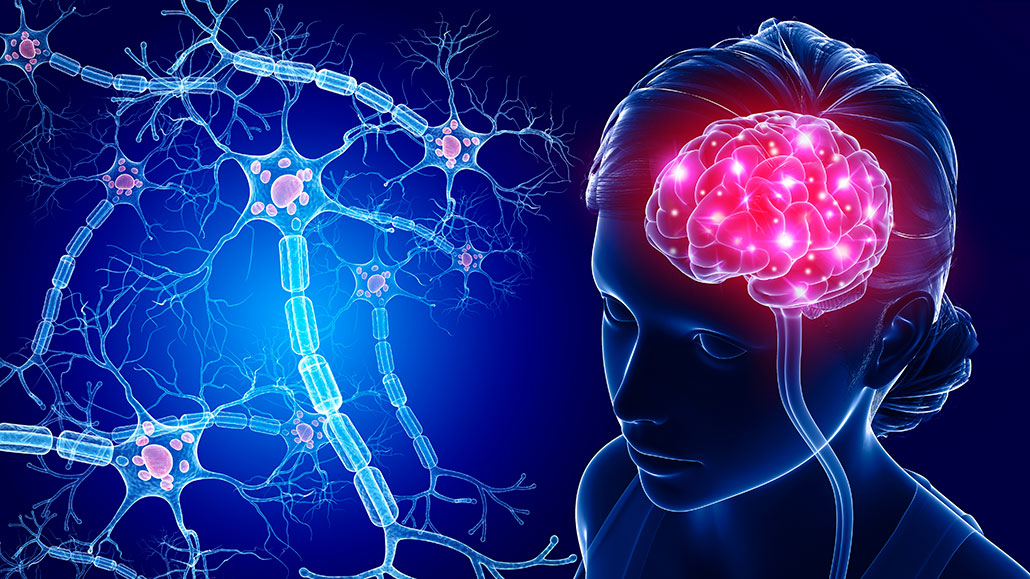
\includegraphics[width=6cm]{neurons.jpg}
  \vspace{-0.8cm}
  \caption{Neuroner i menneskehjernen fra \parencite{St_Clair_2021}}
  \label{fig:neurons}
  \vspace{0.5cm}
  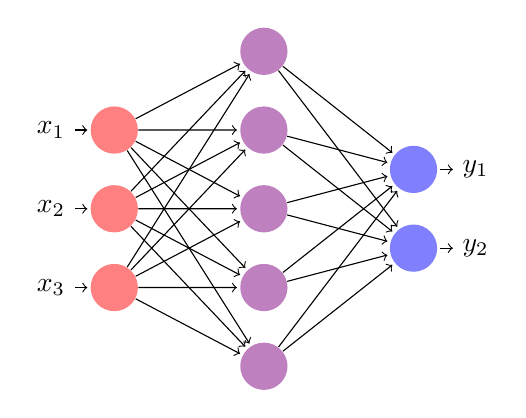
\begin{tikzpicture}

% Input Layer
\foreach \i in {1,...,\inputnum}
{
  \node[circle, 
    minimum size = 6mm,
    fill=red!50] (Input-\i) at (0,-\i) {};
}

% Hidden Layer
\foreach \i in {1,...,\hiddennum}
{
  \node[circle, 
    minimum size = 6mm,
    fill=violet!50,
    yshift=(\hiddennum-\inputnum)*5 mm
  ] (Hidden-\i) at (1.9,-\i) {};
}

% Output Layer
\foreach \i in {1,...,\outputnum}
{
  \node[circle, 
    minimum size = 6mm,
    fill=blue!50,
    yshift=(\outputnum-\inputnum)*5 mm
  ] (Output-\i) at (3.8,-\i) {};
}

% Connect neurons In-Hidden
\foreach \i in {1,...,\inputnum}
{
  \foreach \j in {1,...,\hiddennum}
  {
    \draw[->, shorten >=1pt] (Input-\i) -- (Hidden-\j);	
  }
}

% Connect neurons Hidden-Out
\foreach \i in {1,...,\hiddennum}
{
  \foreach \j in {1,...,\outputnum}
  {
    \draw[->, shorten >=1pt] (Hidden-\i) -- (Output-\j);
  }
}

% Inputs
\foreach \i in {1,...,\inputnum}
{            
  \draw[<-, shorten <=1pt] (Input-\i) -- ++(-0.5,0)
    node[left]{$x_{\i}$};
}

% Outputs
\foreach \i in {1,...,\outputnum}
{            
  \draw[->, shorten <=1pt] (Output-\i) -- ++(0.5,0)
    node[right]{$y_{\i}$};
}

\end{tikzpicture}

  \vspace{-0.8cm}
  \caption{Et simpelt neuralt netværk}
  \label{fig:neural_network}
  \vspace{0.5cm}
  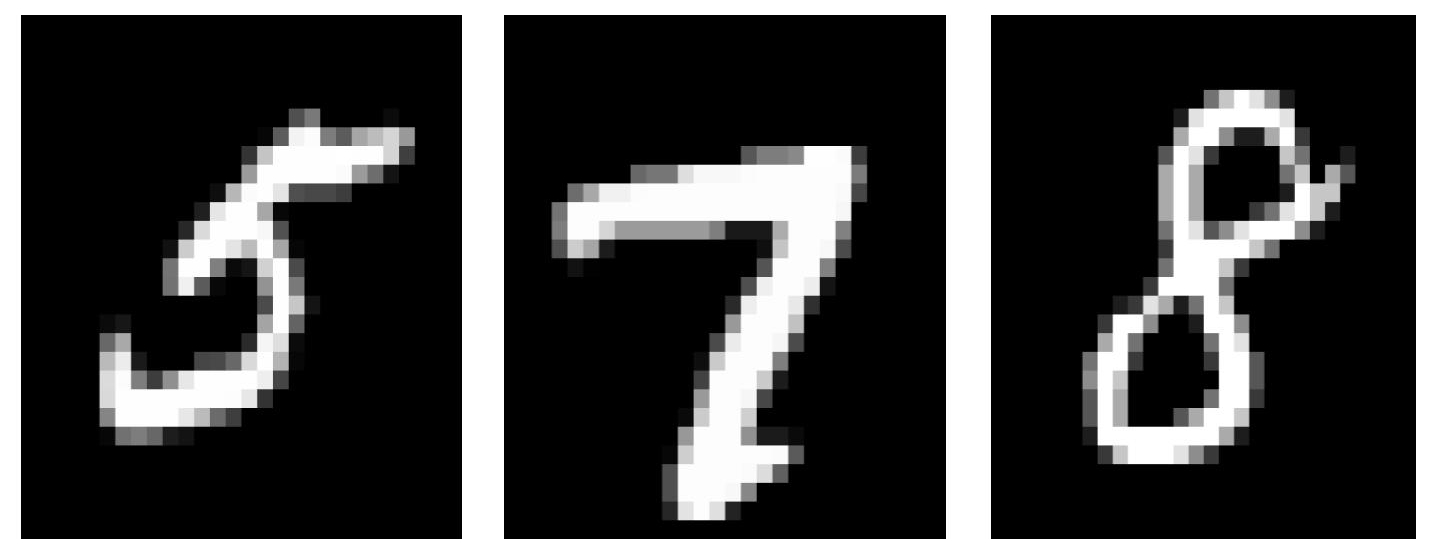
\includegraphics[width=6cm]{mnist1.jpg}
  \vspace{-0.8cm}
  \caption{Eksempel fra MNIST datasættet \parencite{LeCun_1994}}
  \label{fig:mnist}
\end{wrapfigure}
Et neuralt netværk er en matematisk model, der er inspireret af de biologiske neuroner i menneskehjernen. Et neuralt netværk består af en række lag, hvor hvert lag består af neuroner. Dette kan ses på \figureref{fig:neural_network}. Hvert neuron i et lag er forbundet til alle neuroner i det forrige lag og det næste lag. Hver forbindelse mellem neuronerne har en vægt, der bestemmer, hvor meget signalet fra det ene neuron påvirker det næste neuron. Hvert neuron har også en bias, der bestemmer, hvor let det er for neuronet at sende et signal. Et neuralt netværk består af et \color{red!90}inputlag\color{black}, et eller flere \color{violet!90}skjulte lag \color{black} og et \color{blue!90}outputlag\color{black}. Dette er illustreret på \figureref{fig:neural_network}. Det er altså denne model, der er inspireret af de mange sammenkoblede neuroner i menneskehjernen. Denne lighed er ikke tilfældig, da neurale netværk er designet til at efterligne hjernens evne til at lære.\\
Bemærk \figureref{fig:mnist}. Du ved udmærket godt, hvilke tal der er på billedet, selvom du aldrig før har set netop dette 5-, 7- og 8-tal før. Dette er, fordi din hjerne er trænet til at genkende tal. Denne opgave er enormt udfordrende for et alment computerprogram, idet det ikke har nogen intuitiv forståelse af, hvad et tal er, og det skal derfor programmeres med specifikke instruktioner for at kunne genkende tal. Denne tilgang er ikke optimal, da den kræver, at programmøren har en dyb forståelse af, hvordan tal ser ud, og hvordan de kan genkendes. Denne metode er ikke holdbar i længden, idet der er uendeligt mange måder at skrive et 7-tal på. For at kunne generalisere talgenkendelse og gøre metoden mere robust overfor nye skrivemåder af tal kan neurale netværk anvendes. Antag et neuralt netværk med et tal som input og de helt rigtige vægte og biases. Denne model vil i teorien kunne genkende tal, også selvom modellen aldrig før har set netop dette tal. Håbet er, at modellen har "lært" at generalisere træningsdataen til en mere generel forståelse af tal. Modellens output vil derfor være en søjlevektor med sandsynligheder for, at inputtet er et tal fra 0 til 9. Modellens prediktering vil være det tal, der har den højeste sandsynlighed ifølge modellen.
\clearpage
\subsubsection{Feedforward}
Når modellen skal prediktere, altså gå fra input til output, kaldes dette for \textit{feedforward}. Her sendes inputtet gennem alle lagene i modellen, og bliver bliver påvirket af vægtene mellem neuronerne og biaset i hvert neuron. Herunder er et simpelt neuralt netværk med kun 1 neuron i hvert lag og et skjult lag og hvor $a_n$ er aktiveringen af neuronen i lag $n$ og $w_n$ er vægten mellem neuronen i lag $n$ og lag $n+1$:
\begin{center}
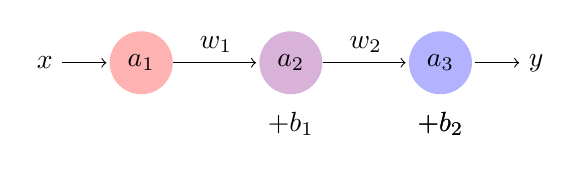
\begin{tikzpicture}
  \node[circle, minimum size=8mm, fill=red!30] (Input-1) at (0,0) {$a_1$};  % Input Layer
  \node[circle, minimum size=8mm, fill=violet!30] (Hidden-1) at (1.9,0) {$a_2$};  % Hidden Layer
  \node[below=0.1cm of Hidden-1] (Hidden-1-bias) {$+b_1$};
  \node[circle, minimum size=8mm, fill=blue!30] (Output-1) at (3.8,0) {$a_3$};  % Output Layer
  \node[below=0.1cm of Output-1] (Output-1-bias) {$+b_2$};
  \node[below=0.1cm of Output-1] {$+b_2$};
  \draw[->, shorten >=1pt] (Input-1) -- (Hidden-1) node[midway, above]{$w_1$};  % Connect neurons
  \draw[->, shorten >=1pt] (Hidden-1) -- (Output-1) node[midway, above]{$w_2$};  % Connect neurons
  \draw[<-, shorten <=1pt] (Input-1) -- ++(-1,0) node[left]{$x$};  % Inputs
  \draw[->, shorten <=1pt] (Output-1) -- ++(1,0) node[right]{$y$};  % Outputs
\end{tikzpicture}
\captionof{figure}{Et simpelt neuralt netværk}
\label{fig:neural_network2}
\end{center}
Så hvis vi ønsker at prediktere outputtet $y$ givet inputtet $x$, så kan vi gøre dette ved at følge disse trin: \\
\begin{align}
a_1 &= x
\\
a_2 &= \sigma(w_1 \cdot a_1 + b_1)
\\
a_3 &= \sigma(w_2 \cdot a_2 + b_2)
\\
y &= a_3
\end{align}
Her er $\sigma(x)$ en aktiveringsfunktion, der tager inputtet $x$ og returnerer et output. Denne funktion er essentiel for at modellen kan lære mere komplekse femomener, da den introducerer ikke-linearitet i modellen. En af de mest brugte aktiveringsfunktioner er ReLU, der tager inputtet $x$ og returnerer $x$ hvis $x > 0$ og 0 ellers. \parencite{Sanderson_2017} Hvis outputtet skal betragtes som en sandsynlighed, er sigmoid funktionen en god aktiveringsfunktion, da den tager inputtet $x$ og returnerer en værdi mellem 0 og 1, som kan tolkes som en sandsynlighed. Sigmoid funktionens definition samt et plot af funktionen er vist herunder: \parencite{Nielsen_2019a}\\
\begin{minipage}{0.4\textwidth}
  \begin{align}
    \sigma(x) = \frac{1}{1 + e^{-x}}
  \end{align}
\end{minipage}
\begin{minipage}{0.6\textwidth}
  \begin{center}
    \begin{tikzpicture}
      \draw[->] (-3,0) -- (3,0) node[right]{$x$};
      \draw[->] (0,-0.5) -- (0,1.5) node[above]{$\sigma(x)$};
      \foreach \x in {-3,-2,-1,1,2,3}
        \draw (\x,0.05) -- (\x,-0.05) node[below] {\x};
      \foreach \y in {1}
        \draw (0.05,\y) -- (-0.05,\y) node[left] {\y};
      \draw[domain=-3:3,smooth,variable=\x,red] plot ({\x},{1/(1 + exp(-\x))});
    \end{tikzpicture}
    \captionof{figure}{Sigmoid funktionen}
    \label{fig:sigmoid}
  \end{center}
\end{minipage}
Typisk har et neuralt netværk flere neuroner i hvert lag, og antallet af vægte og biases er derfor meget større. $x$, $y$, samt alle de forskellige $a_n$ og $b_n$ for hvert lag er søjlevektorer, og $w_n$ i alle lag er matricer. og derfor skal der bruges matrixmultiplikation for at kunne beregne outputtet. Dette er ikke et problem, da de pågældende regneoperationer er defineret tidligere i afsnittet.  

\subsubsection{Træning af neurale netværk}
Når et neuralt netværk initialiseres, er alle vægtene og biases tilfældige. \parencite{Sanderson_2017} Dette betyder, at modellen ikke kan genkende noget, ligesom et barn, der skal lære noget for første gang. For at lære modellen at genkende tal, skal modellen trænes. Dette kræver en anstændig mængde træningsdata og associerede labels, der fortæller modellen, hvad hvert billede er. For at træne modellen skal man vide hvor god modellen er til at prediktere datasættet, en primitiv måde at gøre det på er at angive procenten af rigtigt predikterede tal. Denne metode er ikke velfungerende, da en lille ændring i vægtene og biases vil ændre modellens præstation minimalt og er derfor ikke målbar. For at kunne træne modellen effektivt skal vi vide præcist hvordan en lille ændring i vægtene og biases påvirker modellens præstation. Denne funktion kaldes en \textit{loss funktion}, og er essentiel for at kunne træne modellen. Loss funktionen er en funktion, der tager modellens prediktion og sammenligner den med det rigtige svar. Loss funktionen er en måde at kvantificere, hvor god modellen er til at prediktere. Hvis loss funktionen er høj, er modellen dårlig til at prediktere, og hvis loss funktionen er lav, er modellen god til at prediktere. Herunder ses et eksempel på en loss funktion på et enkelt datapunkt $i$ \parencite{Sanderson_2017}:
\begin{wrapfigure}[5]{r}{4cm}
  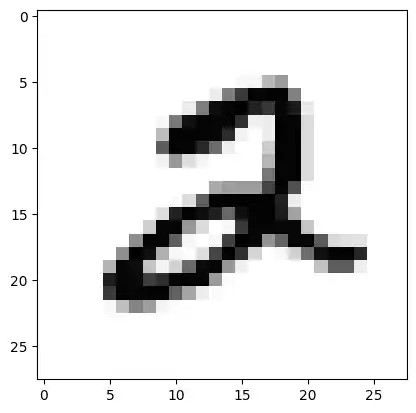
\includegraphics[width=4cm]{mnist2.jpg}
  \vspace{-0.8cm}
  \caption{Eksempel på et 2-tal fra MNIST datasættet \parencite{LeCun_1994}}
  \label{fig:mnist2}
\end{wrapfigure}
\begin{align}
  \underbrace{y_i = \begin{bmatrix}
    0.12 \\
    0.03 \\
    0.25 \\
    0.07 \\
    0.18 \\
    0.09 \\
    0.04 \\
    0.11 \\
    0.06 \\
    0.05
  \end{bmatrix}}_{\text{Modellens prediktion}}
  &&
  \underbrace{\hat{y}_i = \begin{bmatrix}
    0 \\
    0 \\
    1 \\
    0 \\
    0 \\
    0 \\
    0 \\
    0 \\
    0 \\
    0
  \end{bmatrix}}_{\text{Det rigtige svar}}
\end{align}
Loss funktionen for dette datapunkt er den kvadrerede forskel mellem modellens prediktion og det rigtige svar:
\begin{align}
  L_i = (\hat{y} - y_i)^2 = \begin{bmatrix}
    0 - 0.12 \\
    0 - 0.03 \\
    1 - 0.25 \\
    \vdots \\
    0 - 0.05
  \end{bmatrix}^2 = \begin{bmatrix}
    -0.12^2 \\
    -0.03^2 \\
    0.75^2 \\
    \vdots \\
    -0.05^2
  \end{bmatrix}
\end{align}
Nu tages summen af den kvadrerede forskel for at få loss funktionen for dette datapunkt:
\begin{align}
  L_i &= \sum_{i=1}^{10} (\hat{y}_i - y_i)^2\\
      &= (-0.12^2) + (-0.03^2) + (0.75^2) + \ldots + (-0.05^2)
\end{align}
Denne operation gentages for alle datapunkter i træningssættet, og summen tages, derefter divideres summen med antallet af datapunkter for at få gennemsnittet af loss funktionen for hele træningssættet \parencite{Sanderson_2017}:
\begin{align}
  L = \frac{1}{N} \sum_{i=1}^{N} \sum_{j=1}^{10} (\hat{y}_{ij} - y_{ij})^2
\end{align}
Nu har vi en loss funktion, der kvantificerer, hvor god modellen er til at prediktere, og hvor selv en lille ændring i vægtene og biases vil ændre loss funktionen. Nu er det muligt at træne modellen ved at minimere loss funktionen, da man kan sige at når loss funktionen er lav, er modellen god til at prediktere. Desuden er denne loss funktion kontinuert og \text{diff}erentiabel, hvilket er essentielt for at kunne træne modellen. For at minimere loss funktionen bruges en algoritme kaldet \textit{gradient descent}.

\subsection{Softmax}
Softmax er en aktiveringsfunktion, der bruges i det sidste lag af et neuralt netværk, når outputtet skal repræsentere en sandsynlighedsfordeling over forskellige klasser. Softmax-funktionen tager en vektor af vilkårlige reelle tal og omdanner dem til en vektor af sandsynligheder, hvor summen af sandsynlighederne er 1. Softmax-funktionen er defineret som:
\begin{align}
  \text{softmax}(z_i) = \frac{e^{z_i}}{\sum_{j=1}^{K} e^{z_j}}
\end{align}
hvor $z_i$ er elementet i inputvektoren, og $K$ er antallet af klasser. Softmax-funktionen anvendes ofte i klassifikationsproblemer, hvor outputtet skal repræsentere sandsynligheden for hver klasse. Herunder ses et eksempel på softmax-funktionen anvendt på et enkelt datapunkt $i$:
\begin{align}
  \underbrace{\hat{y}_i = \text{softmax}\left(\begin{bmatrix}
    2.0 \\
    1.0 \\
    0.1
  \end{bmatrix}\right)}_{\text{Modellens prediktion}}
  = \begin{bmatrix}
    \frac{e^{2.0}}{e^{2.0} + e^{1.0} + e^{0.1}} \\
    \frac{e^{1.0}}{e^{2.0} + e^{1.0} + e^{0.1}} \\
    \frac{e^{0.1}}{e^{2.0} + e^{1.0} + e^{0.1}}
  \end{bmatrix}
  = \begin{bmatrix}
    0.659 \\
    0.242 \\
    0.099
  \end{bmatrix}
\end{align}
I dette eksempel er sandsynligheden for klasse 1 (første element) 65.9\%, for klasse 2 (andet element) 24.2\%, og for klasse 3 (tredje element) 9.9\%. Softmax-funktionen sikrer, at summen af sandsynlighederne er 1, hvilket gør det muligt at tolke outputtet som en sandsynlighedsfordeling. \parencite{Sanderson_2017}

\subsection{Gradient descent}
Gradient descent er en algoritme, der tager loss-funktionen og beregner gradienten af denne i forhold til alle modellens parametre (vægtene og biases). Gradienten er en vektor, der peger i retningen af den største stigning af loss-funktionen. For at minimere loss-funktionen skal vi derfor bevæge os i den modsatte retning af gradienten. Dette gøres ved at opdatere vægtene og biases i modellen med gradienten ganget med en konstant, kaldet \textit{learning rate}. Processen gentages, indtil loss-funktionen er tilstrækkeligt minimeret. \parencite{IBM_2021, Sanderson_2017, Nielsen_2019a} Antag, at vi organiserer modellens vægte og biases i en søjlevektor $\vec{W}$, og at loss-funktionen er $L(\vec{W})$. Gradienten af loss-funktionen er $\nabla L(\vec{W})$. Derfor beskriver søjlevektoren $-\nabla L(\vec{W})$, hvordan vi kan opdatere $\vec{W}$ for at minimere loss-funktionen og dermed forbedre modellens præstation. Algoritmen, der finder gradienten på baggrund af modellens parametre og loss-funktionen, kaldes \textit{backpropagation}. \parencite{Sanderson_2017, Nielsen_2019a} Hvordan backpropagation fungerer, vil blive gennemgået mere detaljeret i et kommende afsnit. Indtil videre antager vi blot, at den fungerer som beskrevet og returnerer den korrekte gradient for modellens parametre.

\subsection{Partielle afledte}
Partielle afledte bruges til at beskrive, hvordan en funktion ændrer sig, når kun én af dens variabler ændres, mens de andre holdes konstante. Lad os antage, at vi har en funktion $f(x, y)$, der afhænger af to variabler $x$ og $y$. Den partielle afledte af $f$ med hensyn til $x$ betegnes som $\frac{\partial f}{\partial x}$ og repræsenterer hældningen af $f$ i $x$-retningen. Tilsvarende betegner $\frac{\partial f}{\partial y}$ hældningen i $y$-retningen. Partielle afledte er særligt nyttige i optimering og machine learning, hvor de bruges til at finde gradienten af en funktion med flere variabler. Gradientens komponenter består netop af de partielle afledte for hver variabel. For eksempel, hvis vi ønsker at minimere en funktion $f(x, y)$, kan vi bruge gradienten $\nabla f(x, y)$, som indeholder de partielle afledte $\frac{\partial f}{\partial x}$ og $\frac{\partial f}{\partial y}$, til at navigere mod lavere værdier af $f$. \parencite{Kirsanov_2024}

\subsection{Kædereglen}
Kædereglen er en fundamental regel i \text{diff}erentialregning, der gør det muligt at \text{diff}erentiere sammensatte funktioner. Hvis vi har to funktioner, $f(g(x))$, hvor $f$ afhænger af $g(x)$, og $g$ afhænger af $x$, siger kædereglen, at den afledte af $f$ med hensyn til $x$ er produktet af den afledte af $f$ med hensyn til $g$ og den afledte af $g$ med hensyn til $x$:
\begin{align}
  \frac{d}{dx} f(g(x)) = f'(g(x)) \cdot g'(x)
\end{align}
Med Leibniz notation kan kædereglen skrives som:
\begin{align}
  \frac{\partial f}{\partial x} = \frac{\partial f}{\partial z} \cdot \frac{\partial z}{\partial x}
  &&
  \text{hvor } z = g(x)
\end{align}
Kædereglen er en central den i neurale netværk og i machine learning, især i algoritmen backpropagation, hvor det kræves at beregne gradienten af en sammensat loss-funktion i forhold til modellens parametre. \parencite{Kirsanov_2024}
\subsection{Backpropagation}
Antag et simpelt neuralt netværk som det, der er vist i \figureref{fig:neural_network2} tidligere, og loss-funktionen for dette netværk, $L$. $L$ har som funktionsparameter alle modellens parametre og giver en kvantitativ vurdering af, hvor gode disse parametre er givet et datasæt. En primitiv måde at optimere modellens parametre på er at ændre hver parameter separat og undersøge, om loss-funktionen er højere eller lavere med de nye parametre. Hvis loss er lavere, ændres parameteren; hvis ikke, nulstilles parameteren, og den næste justeres. Gentages denne proces tilstrækkeligt mange gange, vil man nærme sig et minimum i loss-funktionen. Selvom denne metode er primitiv, kan den fungere for en simpel model som den, der er visualiseret i \figureref{fig:neural_network2}. Dog vil denne tilgang være ineffektiv og ekstremt langsom for en model med hundredevis eller tusindvis af parametre og er derfor ikke en praktisk metode for den gældende problemstilling. Denne vilkårlige permutationsalgoritme er den bedste metode i generelle tilfælde, da der ikke nødvendigvis findes en bedre metode. \parencite{Kirsanov_2024} For \text{diff}erentiable udregninger, som dem i et neuralt netværk, findes der dog en langt bedre metode, der muliggør markant mere effektiv optimering af modellens parametre. Denne algoritmes formål er at forudsige, hvordan en ændring i modellens parametre vil påvirke loss-funktionen, uden at justere manuelt. Selvom denne algoritme kan lyde umulig, bygger den faktisk på fundamentale matematiske principper. Algoritmen kaldes \textit{backpropagation}. \parencite{Kirsanov_2024, Nielsen_2019b, Sanderson_2017} eksemplet herunder gennemgår hvordan de afledte udregnes i et simpelt neuralt netværk for at illustrere backpropagation anvendt.
\subsubsection{Udregning af gradienten}
Beskue det nedstående neurale netværk med 1 neuron i hvert lag og et skjult lag, Dette afsnit har til formål at gennemgå hvordan gradienten af loss funktionen udregnes i forhold til vægtene og biases i modellen.
\begin{center}
  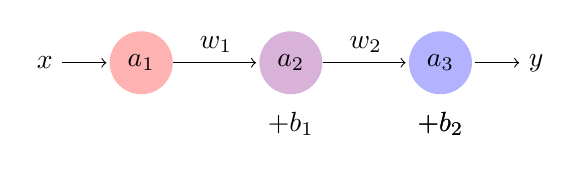
\begin{tikzpicture}
  \node[circle, minimum size=8mm, fill=red!30] (Input-1) at (0,0) {$a_1$};  % Input Layer
  \node[circle, minimum size=8mm, fill=violet!30] (Hidden-1) at (1.9,0) {$a_2$};  % Hidden Layer
  \node[below=0.1cm of Hidden-1] (Hidden-1-bias) {$+b_1$};
  \node[circle, minimum size=8mm, fill=blue!30] (Output-1) at (3.8,0) {$a_3$};  % Output Layer
  \node[below=0.1cm of Output-1] (Output-1-bias) {$+b_2$};
  \node[below=0.1cm of Output-1] {$+b_2$};
  \draw[->, shorten >=1pt] (Input-1) -- (Hidden-1) node[midway, above]{$w_1$};  % Connect neurons
  \draw[->, shorten >=1pt] (Hidden-1) -- (Output-1) node[midway, above]{$w_2$};  % Connect neurons
  \draw[<-, shorten <=1pt] (Input-1) -- ++(-1,0) node[left]{$x$};  % Inputs
  \draw[->, shorten <=1pt] (Output-1) -- ++(1,0) node[right]{$y$};  % Outputs
\end{tikzpicture}
  \captionof{figure}{Et simpelt neuralt netværk}
  \label{fig:neural_network3}
\end{center}
For at simplificere senere udregninger, er modellen konstrueret således at kun $a_2$ benytter sig af en aktiveringsfunktion $\sigma(x)$. Så for at udregne $y$ givet $x$ kan denne udregnes således:
\begin{align}
  y= \sigma(w_1 \cdot x + b_1) \cdot w_2 + b_2  
\end{align}
Og lavet om til en funktion $f(x)$:
\begin{align}
  f(w_1, b_1, w_2, b_2, x) = \sigma(w_1 \cdot x + b_1) \cdot w_2 + b_2
\end{align}
Og insættes i loss funktionen $L(y)$:
\begin{align}
  L&(y) &&= (y - \hat{y})^2 && \text{hvor } \hat{y} \text{ er det rigtige svar}\\
  L&(f(w_1, b_1, w_2, b_2, x)) &&= L(\sigma(w_1 \cdot x + b_1) \cdot w_2 + b_2 - \hat{y})^2
  \label{eq:full_loss}
\end{align}
Hvis vi nu har en loss funktion $L(y)$, der kvantificerer, hvor god modellen er til at prediktere, kan vi nu udregne gradienten af $L$ i forhold til $w_1$, $b_1$, $w_2$ og $b_2$. Dette gøres ved at bruge kædereglen til at udregne de partielle afledte af $L$ i forhold til $w_1$, $b_1$, $w_2$ og $b_2$. Først udregnes $\frac{\partial L}{\partial b_2}$\\
Her kan kædereglen bruges til at udregne $\frac{\partial L}{\partial b_2}$:
\begin{align}
  \frac{\partial L}{\partial b_2} = \frac{\partial L}{\partial y} \cdot \frac{\partial y}{\partial b_2}
\end{align}
Lad os først udregne $\frac{\partial L}{\partial y}$, som er den partielle afledte af $L$ i forhold til $y$, denne er relativt simpel at udregne, da $L$ blot kan \text{diff}erentieres på normal vis:
\begin{align}
  \frac{\partial L}{\partial y} = 2 \cdot (y - \hat{y}) = 2y - 2\hat{y}
\end{align}
Og $\frac{\partial y}{\partial b_2}$, som er den partielle afledte af $y$ i forhold til $b_2$, denne er også simpel at udregne, da resten antages at være konstant og derfor ender vi med:
\begin{align}
  \frac{\partial y}{\partial {\color{blue}b_2}} = 1 && L(\overbrace{\sigma(w_1 \cdot x + b_1) \cdot w_2 + {\color{blue}b_2} }^{y}  - \hat{y})^2
\end{align}
Så $\frac{\partial L}{\partial b_2}$ kan nu udregnes:
\begin{align}
  \frac{\partial L}{\partial b_2} &= \frac{\partial L}{\partial y} \cdot \frac{\partial y}{\partial b_2} = \frac{\partial L}{\Ccancel[red]{\partial y}} \cdot \frac{\Ccancel[red]{\partial y}}{\partial b_2}\\
  &= (2y - 2\hat{y}) \cdot 1 = 2y - 2\hat{y} \quad\text{hvor}\quad y = \sigma(w_1 \cdot x + b_1) \cdot w_2 + b_2\\
  &= 2\cdot\sigma(w_1 \cdot x + b_1) \cdot w_2 + 2b_2 - 2\hat{y}
\end{align}
Nu er $\frac{\partial L}{\partial b_2}$ udregnet! Nu kan $\frac{\partial L}{\partial w_2}$ udregnes på samme måde, først opdeles $\frac{\partial L}{\partial w_2}$ efter kædereglen:
\begin{align}
  \frac{\partial L}{\partial w_2} = \frac{\partial L}{\partial y} \cdot \frac{\partial y}{\partial w_2}
\end{align}
Eftersom $\frac{\partial L}{\partial y}$ allerede er udregnet, kan vi nu udregne $\frac{\partial y}{\partial w_2}$, som er den partielle afledte af $y$ i forhold til $w_2$. Dette kan udregnes da $w_2$ kun afhænger af $\sigma(w_1 \cdot x + b_1)$ og da den er konstant i forhold til $w_2$, den partielle afledte er derfor lig $\sigma(w_1 \cdot x + b_1)$:
\begin{align}
  \frac{\partial y}{\partial {\color{blue}w_2}} = \sigma(w_1 \cdot x + b_1) && L(\overbrace{\sigma(w_1 \cdot x + b_1) \cdot {\color{blue}w_2} + b_2}^{y}  - \hat{y})^2
\end{align}
Så $\frac{\partial L}{\partial w_2}$ kan nu udregnes:
\begin{align}
  \frac{\partial L}{\partial w_2} &= \frac{\partial L}{\partial y} \cdot \frac{\partial y}{\partial w_2} = \frac{\partial L}{\Ccancel[red]{\partial y}} \cdot \frac{\Ccancel[red]{\partial y}}{\partial w_2}\\
  &= (2y - 2\hat{y}) \cdot \sigma(w_1 \cdot x + b_1) \quad\text{hvor}\quad y = \sigma(w_1 \cdot x + b_1) \cdot w_2 + b_2\\
  &= 2\cdot(\sigma(w_1 \cdot x + b_1) \cdot w_2 + b_2 - \hat{y}) \cdot \sigma(w_1 \cdot x + b_1)
\end{align}
Nu er $\frac{\partial L}{\partial w_2}$ udregnet! Nu kan $\frac{\partial L}{\partial b_1}$ udregnes på samme måde, Dog er denne mere kompleks, da den er "dybere" i kæden, og derfor skal der bruges kædereglen flere gange. Først opdeles $\frac{\partial L}{\partial b_1}$ efter kædereglen:
\begin{align}
  \frac{\partial L}{\partial b_1} = \frac{\partial L}{\partial y} \cdot \frac{\partial y}{\partial a_2} \cdot \frac{\partial a_2}{\partial b_1}
\end{align}
Beskue \figureref{fig:neural_network3} og Ligning \eqref{eq:full_loss} for hvordan $a_2$ er defineret. Så $\frac{\partial L}{\partial b_1}$ kan nu udregnes, da $\frac{\partial L}{\partial y}$ allerede er udregnet, kan vi nu udregne $\frac{\partial y}{\partial a_2}$, som er den partielle afledte af $y$ i forhold til $a_2$. Her kan samme tankegang bruges idet $a_2$ kun afhænger af $w_2$:
\begin{align}
  \frac{\partial y}{\partial {\color{blue}a_2}} = w_2 && L(\overbrace{{\color{blue}\sigma(w_1 \cdot x + b_1)} \cdot w_2 + b_2}^{y}  - \hat{y})^2
\end{align}
Nu kan $\frac{\partial a_2}{\partial b_1}$ udregnes, som er den partielle afledte af $a_2$ i forhold til $b_1$. Her vil den partielle afledte være $\sigma'(w_1 \cdot x + b_1)$, da $a_2$ afhænger direkte af $b_2$ gennem aktiveringsfunktionen
\begin{align}
  \frac{\partial a_2}{\partial {\color{blue}b_1}} = \sigma'(w_1 \cdot x + b_1) && L(\overbrace{\sigma(w_1 \cdot x + {\color{blue}b_1})}^{a_2} \cdot w_2 + b_2 - \hat{y})^2
\end{align}
Så $\frac{\partial L}{\partial b_1}$ kan nu udregnes:
\begin{align}
  \frac{\partial L}{\partial b_1} &= \frac{\partial L}{\partial y} \cdot \frac{\partial y}{\partial a_2} \cdot \frac{\partial a_2}{\partial b_1} = \frac{\partial L}{\Ccancel[red]{\partial y}} \cdot \frac{\Ccancel[red]{\partial y}}{\Ccancel[red]{\partial a_2}} \cdot \frac{\Ccancel[red]{\partial a_2}}{\partial b_1}\\
  &= (2y - 2\hat{y}) \cdot w_2 \cdot \sigma'(w_1 \cdot x + b_1) \quad\text{hvor}\quad y = \sigma(w_1 \cdot x + b_1) \cdot w_2 + b_2\\
  &= 2\cdot(\sigma(w_1 \cdot x + b_1) \cdot w_2 + b_2 - \hat{y}) \cdot w_2 \cdot \sigma'(w_1 \cdot x + b_1)
\end{align}
Nu er $\frac{\partial L}{\partial b_1}$ udregnet! Nu kan $\frac{\partial L}{\partial w_1}$ udregnes på samme måde, På samme måde er denne mere kompleks, da den også er "dybere" i kæden, og derfor skal der bruges kædereglen flere gange. Først opdeles $\frac{\partial L}{\partial w_1}$ efter kædereglen:
\begin{align}
  \frac{\partial L}{\partial w_1} = \frac{\partial L}{\partial y} \cdot \frac{\partial y}{\partial a_2} \cdot \frac{\partial a_2}{\partial w_1}
\end{align}
Så $\frac{\partial L}{\partial w_1}$ kan nu udregnes, da $\frac{\partial L}{\partial y}$ og $\frac{\partial y}{\partial a_2}$ allerede er udregnet, Nu kan $\frac{\partial a_2}{\partial w_1}$ udregnes, som er den partielle afledte af $a_2$ i forhold til $w_1$. Da $a_2 = \sigma(w_1 \cdot x + b_1)$, afhænger $a_2$ af $w_1$ gennem argumentet, og derfor vil den partielle afledte være:
\begin{align}
  \frac{\partial a_2}{\partial {\color{blue}w_1}} = x \cdot \sigma'(w_1 \cdot x + b_1) && L(\overbrace{\sigma({\color{blue}w_1} \cdot x + b_1)}^{a_2} \cdot w_2 + b_2  - \hat{y})^2
\end{align}
Så $\frac{\partial L}{\partial w_1}$ kan nu udregnes:
\begin{align}
  \frac{\partial L}{\partial w_1} &= \frac{\partial L}{\partial y} \cdot \frac{\partial y}{\partial a_2} \cdot \frac{\partial a_2}{\partial w_1} = \frac{\partial L}{\Ccancel[red]{\partial y}} \cdot \frac{\Ccancel[red]{\partial y}}{\Ccancel[red]{\partial a_2}} \cdot \frac{\Ccancel[red]{\partial a_2}}{\partial w_1}\\
  &= (2y - 2\hat{y}) \cdot w_2 \cdot x \cdot \sigma'(w_1 \cdot x + b_1) \quad\text{hvor}\quad y = \sigma(w_1 \cdot x + b_1) \cdot w_2 + b_2\\
  &= 2\cdot(\sigma(w_1 \cdot x + b_1) \cdot w_2 + b_2 - \hat{y}) \cdot w_2 \cdot x \cdot \sigma'(w_1 \cdot x + b_1)
\end{align}
Lad os tage et skridt tilbage og opsummere, hvad der er blevet udregnet. Vi har nu udregnet gradienten af loss funktionen i forhold til modellens parametre, netop $w_1$, $b_1$, $w_2$ og $b_2$. Dette er essentielt for at kunne træne modellen effektivt, da vi nu ved, hvordan loss funktionen ændrer sig, når vi ændrer vægtene og biases. Dette gør det muligt at bruge gradient descent til at minimere loss funktionen og dermed forbedre modellens præstation. Dette gøres i priksis ved at gemme mellenregningerne når modellen prediktere, og derefter bruge disse mellemregninger til at regne baglæns og dermed finde gradienten, det er her algoritmen backpropagation får sit navn. Selvom eksemplet i dette afsnit er simpelt, kan samme principper anvendes på langt mere komplekse neurale netværk med mange flere lag og neuroner. her vil værdierne dog være matricer og vektorer, og derfor vil de partielle afledte således også være organiseret i matricer, mens dette lyder komplekst, er det i praksis blot en udvidelse af de principper, der er blevet gennemgået i dette afsnit, bare med flere indekser.\\\\
Lad os for en god ordens skyld tjekke vores svar efter ved brug af Maple CAS værktøjet:
\begin{align}
  L(y)&\coloneqq(y-\hat{y})^{2}\colon\\
  f(w_{1},b_{1},w_{2},b_{2},x)&\coloneqq\sigma(w_{1}\cdot x+b_{1})\cdot w_{2}+b_{2}\colon\\
  \frac{\partial L}{\partial b_{2}}=\text{diff}(L(f(w_{1},b_{1},w_{2},b_{2},x)),b_2)&=\color{blue}2\cdot\sigma(w_{1}\cdot x+b_{1})\cdot w_{2}+2\cdot b_{2}-2\cdot\hat{y}\\
  \frac{\partial L}{\partial w_{2}}= \text{diff}(L(f(w_{1},b_{1},w_{2},b_{2},x)),w_2)&=\color{blue}2\cdot(\sigma(w_{1}\cdot x+b_{1})\cdot w_{2}+b_{2}-\hat{y})\cdot\sigma(w_{1}\cdot x+b_{1})\\
  \frac{\partial L}{\partial b_{1}}= \text{diff}(L(f(w_{1},b_{1},w_{2},b_{2},x)),b_1)&=\color{blue}2\cdot(\sigma(w_{1}\cdot x+b_{1})\cdot w_{2}+b_{2}-\hat{y})\cdot w_{2}\cdot\sigma'(w_{1}\cdot x+b_{1})\\
  \frac{\partial L}{\partial w_{1}}= \text{diff}(L(f(w_{1},b_{1},w_{2},b_{2},x)),w_1)&=\color{blue}2\cdot(\sigma(w_{1}\cdot x+b_{1})\cdot w_{2}+b_{2}-\hat{y})\cdot w_{2}\cdot x\cdot\sigma'(w_{1}\cdot x+b_{1})
\end{align}
Som det ses er vores svar korrekt, og dermed er vores udregninger korrekte. 
\section{Valg af programmeringssprog}
Til at implementere et neuralt netværk, er det nødvændigt at vælge et programmeringssprog, der er egnet til formålet. Der findes mange forskellige programmeringssprog, der kan bruges til at implementere neurale netværk, herunder Python, R, Java, C++, og mange flere. Men da det ønskes at programmet er interaktivt og let at bruge, er Python med PyGame eller Java med Processing de mest oplagte valg. Python og mere specifikt NumPy, som er et bibliotek til Python, er enormt brugervenligt og hurtigt at udføre matriceregning i. Java er også et godt valg, da det er et meget populært programmeringssprog, med faste typer som gør det nemmere at undgå fejl. Processing er et bibliotek til Java, der gør det nemt at lave grafik og interaktive applikationer. Men grundet Python's minimale syntaks er det valt til udviklingen af programmet.

\newpage
\printbibliography


\end{document}
